%!TeX root=../tese.tex
%("dica" para o editor de texto: este arquivo é parte de um documento maior)
% para saber mais: https://tex.stackexchange.com/q/78101

%% ------------------------------------------------------------------------- %%

\chapter{Metodologia}
\label{cap:metodologia}

Este estudo de caso se faz com a utilização do \emph{framework} TensorFlow 2.0, uma atualização do TensorFlow original lançada pelo Google\index{Google} em setembro de 2019 ~\citep{TensorFlow2-release}\index{TensorFlow}. A utilização de uma \emph{framework}, como o TensorFlow, simplifica os processos de criação, de treino e de execução do agente inteligente, o que, por um lado, permite um maior investimento energético em melhorar as definição do ambiente e em desenvolver as métricas utilizadas para recompensar ou punir as ações tomadas pelo agente durante o treino, contudo, por outro lado, passa o controle do treino e desenvolvimento do agente para a \emph{framework}, por conseguinte, os transforma em uma caixa preta cujo o funcionamento só é conhecido pelos desenvolvedores de dada \emph{framework}.

Para realizar o treinamento é necessário um computador rodando sistema Linux, preferencialmente Ubuntu uma vez que é o único sistema operacional oficialmente suportado pelo simulador ~\citep{Duckietown-requerimentos}. Dessa forma, este trabalho é desenvolvido na versão 22.04.1 do Ubuntu para processadores de 64-bit, além do uso de GPU GeForce RTX 2060 da Nvidia™ para acelerar o processo ao permitir uma maior paralelização de instâncias de treino e de CPU Intel Core™ i7-8700\footnote{Para a definição de hardware completa consulte o anexo~\ref{annex:hardware}} como visto na figura ~\ref{fig:sobre_computador}. Para o gerenciamento de software usa-se a versão 4.13.0 do Conda ~\citep{Anaconda} que é capaz de controlar a versão do Python além de criar ambientes independentes para cada projeto, e é utilizado o Python 3.10.4, a versão mais recente de Python quando este trabalho foi iniciado.

\begin{figure}
	\centering
	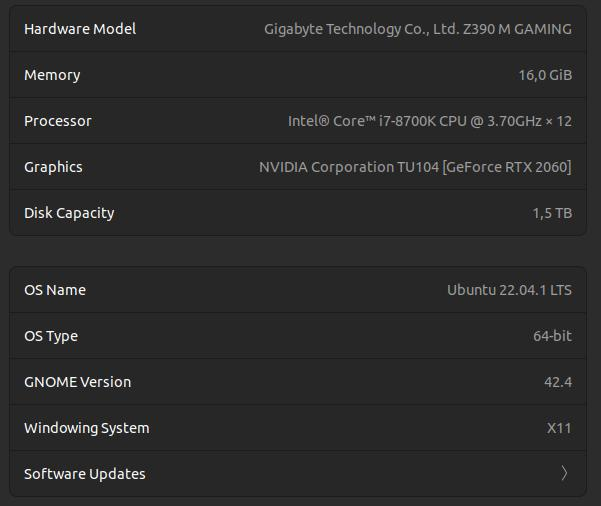
\includegraphics[width=.8\textwidth]{sobre_computador}
	\caption{Informações do sistema. \label{fig:sobre_computador}}
\end{figure}

\section{Critérios de treinamento}
\label{sec:criterios_de_treinamto}

Como em qualquer método de ensino, para realizar um aprendizado por reforço é necessário alguma métrica com a qual se é possível julgar se o comportamento aprendido é bom ou ruim. Desta forma, para este trabalho utiliza de diferentes parâmetros para calcular a pontuação da rede neural durante o treino, em primeiro lugar, é encerrada prematuramente qualquer instância em que o robô saia da pista, pois sair da pista é visto como uma infração gravíssima. Depois, a rede neural recebe uma bonificação pequena por andar do lado certo da pista, uma média por andar em linha reta e uma grande toda vez que o Duckiebot atinge uma nova casa da pista, com a finalidade de incentivar o robô a se mover pelo circuito definido ao invés de ficar girando dentro das mesmas casas da pista. E por último, existe uma punição pequena quando o robô faz curvas, para promover uma maior estabilidade no movimento, uma média quando o robô anda na contra-mão e uma grande quando o ângulo do robô em relação a pista é maior que 40°, cujo o intuito é inibir que ele fique girando na pista ao invés de seguir o circuito.
	
Ademais, as definições da rede neural também são de suma importância para permitir um bom aprendizado por parte da inteligência artificial. Com isso em mente, a rede densa possui 3 camadas, com 100, 75 e 50 nos respectivamentes, e de entrada ela recebe a distância em relação à faixa central da pista, a qual é definida como 1 sendo o limite direito da pista, -1 o limite esquerdo e 0 a faixa central, e o ângulo que o robô está fazendo com a pista, 0 quando ele está paralelo à pista e ± 90 ao estar perpendicular à pista. E por fim, a rede retorna um número inteiro correspondente a ação que deve ser tomada, com o universo das ações possíveis simplificado para 3 diferentes possibilidades: ou ir em frente ou virar à esquerda ou virar à direita; para acelerar o processo de treinamento, uma vez que ele progredia muito lentamente com as 25 possibilidades iniciais.
